\documentclass[twocolumn,10pt]{asme2ej}
\usepackage{epsfig}
\usepackage{graphicx}
\usepackage{amssymb}
\usepackage{enumerate}
\usepackage{enumitem}
\usepackage{float}
% \usepackage{lipsum}
% \usepackage{mathtools}
% \usepackage{subcaption}
% \usepackage{relsize}
% \usepackage{listings}
% \usepackage{color}
\usepackage{hyperref}
% \usepackage{relsize}
% \usepackage{commath}
\usepackage{dirtytalk}
\usepackage{titlesec}
\usepackage{relsize}
\usepackage{amsmath}

\newcommand{\C}{\mathbb{C}}
\newcommand{\I}{\mathbb{I}}
\newcommand{\R}{\mathbb{R}}
\newcommand{\N}{\mathbb{N}}
\newcommand{\K}{\mathbb{K}}

\newcommand{\rd}{\textrm{d}}

\newcommand{\bc}{\textbf{c}}
\newcommand{\bbf}{\textbf{f}}
\newcommand{\bg}{\textbf{g}}
\newcommand{\bu}{\textbf{u}}
\newcommand{\bv}{\textbf{v}}
\newcommand{\bw}{\textbf{w}}
\newcommand{\bx}{\textbf{x}}
\newcommand{\by}{\textbf{y}}


\newcommand{\diag}[1]{\textrm{diag}\left(#1\right)}
\newcommand{\dbyd}[1]{\frac{\rd}{\rd#1}}
\newcommand{\re}[1]{\textrm{Re}\left(#1\right)}
\newcommand{\imag}[1]{\textrm{Im}\left(#1\right)}
\newcommand{\trace}[1]{\textrm{tr}\left(#1\right)}
\newcommand{\deriv}[2]{\dfrac{ d #1}{ d #2}}
\newcommand{\fn}[1]{f_{ #1}}

\renewcommand{\labelenumii}{\theenumii}
\renewcommand{\theenumii}{\theenumi.\arabic{enumii}.}
\newcommand\numberthis{\addtocounter{equation}{1}\tag{\theequation}}
\graphicspath{{figures/}}

\titlespacing\section{0pt}{12pt plus 4pt minus 2pt}{0pt plus 2pt minus 2pt}
\titlespacing\subsection{0pt}{12pt plus 4pt minus 2pt}{0pt plus 2pt minus 2pt}
\titlespacing\subsubsection{0pt}{12pt plus 4pt minus 2pt}{0pt plus 2pt minus 2pt}
% \titlespacing{\section}{0pt}{\parskip}{-\parskip}
% \titlespacing{\subsection}{0pt}{\parskip}{-\parskip}
% \titlespacing{\subsubsection}{0pt}{\parskip}{-\parskip}
\newcommand{\squeezeup}{\vspace{-3mm}}
%\DeclarePairedDelimiter{\ceil}{\lceil}{\rceil} %%for ceil

\title{An Extension of the Swarmalator Model}
%%% first author
\author{Ankith Anil Das
    \affiliation{
    470485327\\
	Faculty of Science, Mathematics\\
	The University of Sydney\\
    Email: aani9804@uni.sydney.edu.au
    }
}


\begin{document}

\maketitle
%
%%%%%%%%%%%%%%%%%%%%%%%%%%%%%%%%%%%%%%%%%%%%%%%%%%%%%%%%%%%%%%%%%%%%%%
\begin{abstract}
{
     \it Synchronization occurs at many natural and technological systems. Such an emergent properties is observed in cardiac pacemaker cells, Japanese tree frogs, colloidal suspensions of magnetic particles, and other biological and technological systems in which synchronization interact. We consider the system where oscillators can sync and swarm. A detailed analysis was proposed by Kevin P. O'Keeffe in the paper \say{Oscillators the sync and swarm}. We studied an extended model of the Swarmalator model proposed in the paper. Understanding the dynamics of this model could possibly give insight to the generalized model where the phase coupling function could be a fourier series.
}
\end{abstract}

% %%%%%%%%%%%%%%%%%%%%%%%%%%%%%%%%%%%%%%%%%%%%%%%%%%%%%%%%%%%%%%%%%%%%%%
% \begin{nomenclature}
% \entry{A}{You may include nomenclature here.}
% \entry{$\alpha$}{There are two arguments for each entry of the nomemclature environment, the symbol and the definition.}
% \end{nomenclature}

% The primary text heading is  boldface and flushed left with the left margin.  The spacing between the  text and the heading is two line spaces.

% %%%%%%%%%%%%%%%%%%%%%%%%%%%%%%%%%%%%%%%%%%%%%%%%%%%%%%%%%%%%%%%%%%%%%%

\section{Introduction}


\noindent
\section{The Model}
{
    We consider swarmalators free to move in the plane. The governing equations are     \noindent
    \begin{equation}
        \dot{\mathbf{x}}_{i}=\mathbf{v}_{i}+\frac{1}{N} \sum_{j=1}^{N}\left[\mathbf{I}_{\mathrm{att}}\left(\mathbf{x}_{j}-\mathbf{x}_{i}\right) F\left(\theta_{j}   -\theta_{i}\right)-\mathbf{I}_{\mathrm{rep}}\left(\mathbf{x}_{j}-\mathbf{x}_{i}    \right)\right]
    \end{equation}
    \begin{equation}
        \dot{\theta}_{i}=\omega_{i}+\frac{K}{N} \sum_{j=1}^{N} H_{\mathrm{att}}\left(\theta_{j}-\theta_{i}\right) G\left(\mathbf{x}_{j}-\mathbf{x}_{i}\right)
    \end{equation}
    for \(i = 1,\ldots,N\), where \(N\) is the number of swarmalators, $\mathbf{x}_{i} $ is the position of the \(i\)-th swarmalator, and $\theta_i,\omega_i,$ and $\mathbf{v}_i$ are it's phase, natural frequency and background velocity. The functions $\mathbf{I}_  {att}$ and $\mathbf{I}_{rep}$ represent spatial attraction and repulsion between the swarmalators where as phase interaction is governed by $\mathbf{H}_{att}$. We considered the following model:
    \begin{equation}
        \dot{\mathbf{x}}_{i}=\mathbf{v}_{i}+\frac{1}{N}\left[\sum_{j \neq i}^{N} \frac  {\mathbf{x}_{j}-\mathbf{x}_{i}}{\left|\mathbf{x}_{j}-\mathbf{x}_{i}\right|}\left  (1+J \cos \left(\theta_{j}-\theta_{i}\right)\right)-\frac{\mathbf{x}_{j}-\mathbf{x}_{i}}{\left|\mathbf{x}_{j}-\mathbf{x}_{i}\right|^{2}}\right]
    \end{equation}
    \begin{equation} \label{eq:phase}
        \dot{\theta}_{i}=\omega_{i}+\frac{K}{N} \sum_{j \neq i}^{N} \frac{\gamma_1 \sin\left(\theta_{j}-\theta_{i}\right) + \gamma_2 \sin \left(2 \left(\theta_j -\theta_i\right)\right) }{\left|\mathbf{x}_{j}-\mathbf{x}_{i}\right|} 
    \end{equation}
    %% State the differences of our model to the original swarmalator model 
    We considered identical swarmalators so that $\omega_i = \omega$ and $\mathbf{v}_i = \mathbf{v}$. Using this assumption, using a suitable choice of reference frame we  can set $\omega = 0$, and $\mathbf{v} = \mathbf{0}$. The system has four parameters $\left(J,K,\gamma_1,\gamma_2\right )$.

    The parameter \(J\) measures the extend to which phase similarity enhances spatial attraction. For $J>0$, swarmalators prefer to be near other swarmalators with  similar phase. When $J<0$, the opposite behavior is observed: swarmalators attract those with opposite phase. When $J=0$, they show no phase based spatial behavior,i.e, their spatial attraction is independent of phase. To maintain $\mathbf{I}_{att}> 0$, we constrain $J$ to $-1 \leq J \leq 1$. The parameter $K$ is the phase coupling strength which scales $\gamma_1$, and $\gamma_2$. The relative  strengths of $\gamma_1$ and $\gamma_2$ determine the stability of one or two clusters. 
    
    Before stating the dynamics of the system, we pause to state the features of this model. This model's purpose is to study the interplay between swarming and synchronization. Our model accounts for aggregation, but not alignment. There are no alignment terms.  We chose to neglect orientation because it adds another layer of complexity; it makes each swarmalator have four state variables. For rest of the report we will refer to our model as `Dual phase coupled model' because of the presence of double angle $\sin$ function in Eq.\ref{eq:phase}. In a similar fashion, the original model proposed by Kevin P. O'Keeffe will be referred as `Single phase coupled model'.\noindent
}
\section{Optimization of the ode solver}
{
    The simulations were run using MATLAB's ODE integrator `ode45'. Absolute and Relative tolerance for the integrator was set to $10^{-6}$. Before large computations were performed, optimisation of the existing code was necessary. As this project involves computations of large matrices using ode45, optimising the code for speed was essential for any extensive calculation. The initial code was profiled using MATLAB's performance profiler, and bottlenecks were identified. Calculating the pairwise inverse distance was the most computationally expensive part in the ode function. The original code took 70 seconds for a simulation with $N = 100$ and $T = 10$-time units. This speed was too slow for any extended time simulations. After removing unwanted function calls, changing the algorithm, and using functions which supports vectorization, the new code took 0.509 sec for the same task. The performance was good enough for an interactive user simulation where the user can change the parameters of the system and can see the results almost instantly.
}
% \section{Single Cluster Stability}
% {

% }

% \noindent
% \section{Two cluster Stability}
% {

% }
% \noindent

\section{Cluster formation and stability}
{
    %One of the core objectives of this project was to understand the cluster formation and its stability.
    The dynamics of dual phase coupled model had some striking differences with the original single phase model. The system not only settled in all the five states which were discussed in detail by Kevin P. O'Keeffe in single phase model, but also showed many additional stable and metastable states. Understanding the behavior of the modified phase coupling term and how it affects the formation of states could give us deep insights about the generalization of the model.
    % Maybe modify this %
    The additional cluster states made by the model can be broadly classified as follows 
    \begin{enumerate}[label = (\alph*)]
        \item Static two cluster state
        \item Two cluster state with rogues 
        \item Active 4 cluster state
        \item Active single cluster state
    \end{enumerate}
    % add figures for the model%
    \noindent
    To understand system behavior under the change of \(\gamma_1\), and \(\gamma_2\), we chose \(J = 0.8\) and \(K = -0.5\) which represent Active phase wave in single phase coupled model. This set of state variables were chosen because it showed the most active spacial behavior in single phase coupled model and the dynamics of the system would be more depended on the values of \(\gamma_1\) and \(\gamma_2\). Unless otherwise stated, the simulations are run with \(J = 0.8\) and \(K = -0.5\). Also, all the simulations were run with random initial position in a 1x1 box and phases from \([-\pi, \pi]\), both uniformly and random. To maintain consistency, the same random seed was used for all simulations.
    \squeezeup
    \begin{figure}[h!]
        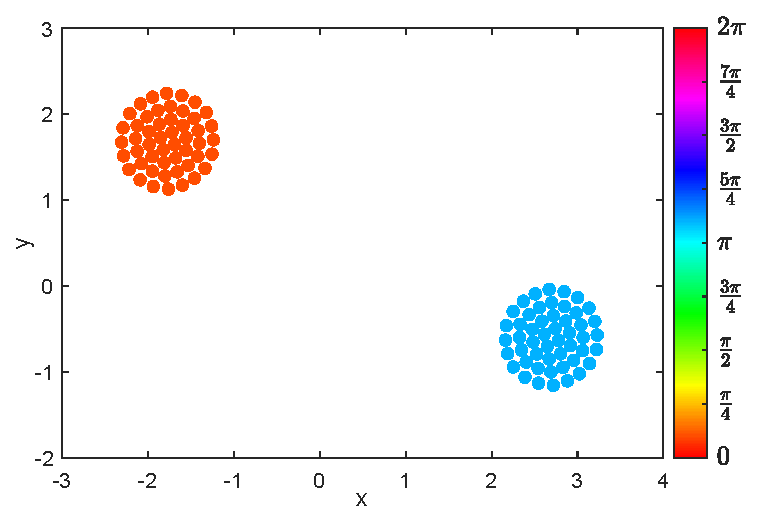
\includegraphics[width = \linewidth]{TwoCluster.eps}
        \caption{Static two Cluster State. This state was achieved for \(N = 100\), \(\gamma_1 = 1/3\), and \(\gamma_2 = -0.5\). The simulation was run for \(T = 100\) time steps with variable step-size (ode45) for the system to settle down.}
        \vspace{-12mm}
        \label{fig:static2}
    \end{figure}
    \begin{figure}[h!]
        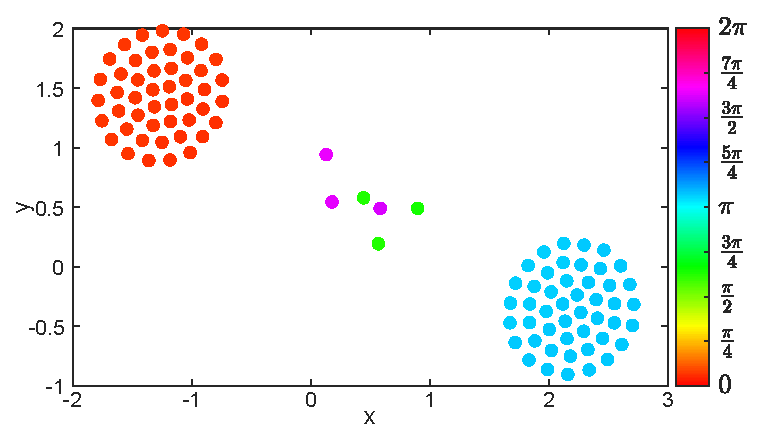
\includegraphics[width = \linewidth]{twoClustersWithR100.eps}
        \caption{Two Clusters with Rogues}
    \end{figure}
    \begin{figure}[h!]
        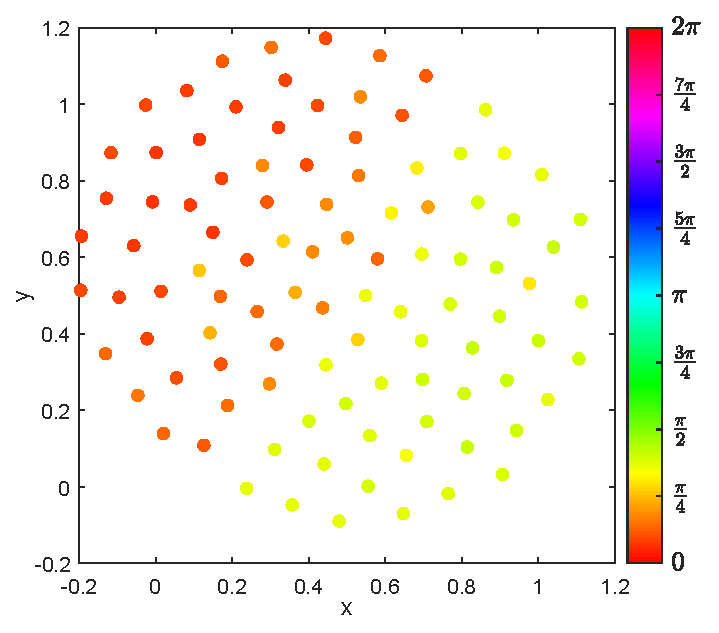
\includegraphics[width = \linewidth]{ActiveSingle.eps}
        \caption{Active Single cluster state}
    \end{figure}
    \begin{figure}
        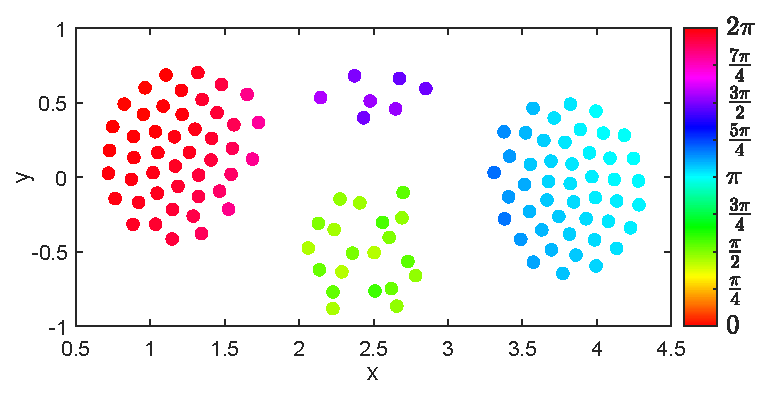
\includegraphics[width = \linewidth]{Active4Clust.eps}
        \caption{Active 4 cluster state}
    \end{figure}
    %% Phase distribution in 2 cluster state. 
    % Show a graph which shows phase with time and how it settles down.
    % Explain why such settling is expected
    % Discuss about the values of K J gamma1 and gamma2 values chosen for the sims 
    % Point out that a detailed explanation for the chosen gamma1 and gamma2 values will be discussed in the later section. 
    % Make a code to find the jacobian matrix and look at the stability of the system
    \subsection{Static Two cluster state}
    {
        \noindent
        Static two cluster case is a very common equilibrium state seen for various values of \((J,K,\gamma_1,\gamma_2)\), illustrated in  Fig.\ref{fig:static2}. Since \(J > 0\), `like attracts like': swarmalators want to settle near other swarmalators with similar phase. Looking at phase dynamics equation (Eq.\ref{eq:phase}) \(\dot{\theta}_{i} = 0\) when \(\theta_i = C, C + \pi \), where \(C\) is any constant. Due to the presence of a new stable phase, the system can form two clusters with \(\pi\) phase difference. Now for the given value of \(K\) which is less than 0, \(\gamma_1 > 0\) (Some coupling) implies the system does not prefer single cluster state, and \(\gamma_2 < 0\) (other coupling) means the system prefers to stabilize in two cluster state. Furthermore, \(|\gamma_2| > |\gamma_1|\) shows that the second coupling term in Eq.\ref*{eq:phase} is more dominant in stabilizing the system. Fig.\ref{fig:phasevsTime} shows how the phase settles with time. Here, the phase effectively stabilizes to two values after taking mod \(2\pi\). The average cluster phase difference is approximately \(\pi\) with an absolute error \(\epsilon \approx 2.6074 \times 10^{-9}\). Our statement about two cluster phase difference can be confirmed with the small error. 

        \begin{figure}
            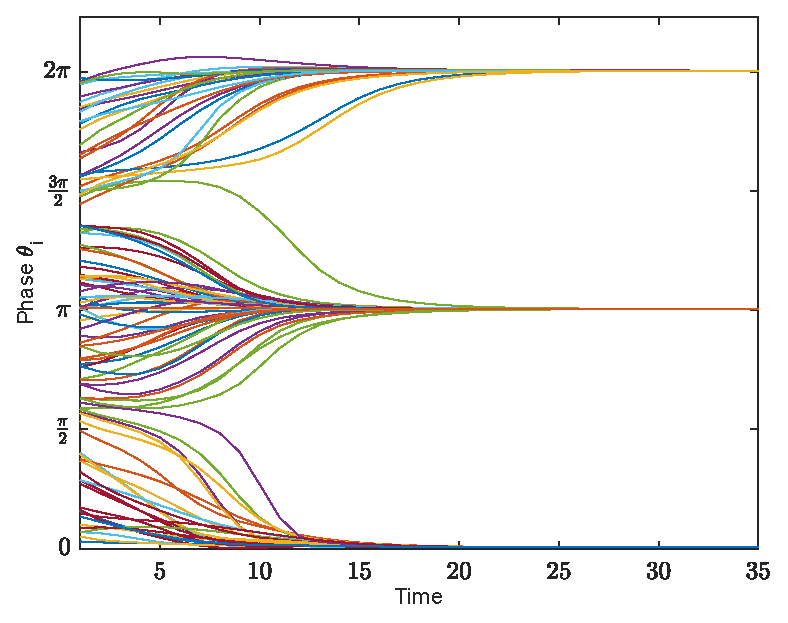
\includegraphics[width = \linewidth]{phasevstimeN_100.eps}
            \caption{Phase of the Swarmalator vs Time. }
            \label{fig:phasevsTime}
        \end{figure}
    }
    
    \subsection{Inter-cluster distance for Static two cluster state}
    {
        We can analytically solve the inter-cluster distance for static two cluster state by making an assumption.
        Let,
        \begin{align} %% Fix this stupid sum SIghISHFISHFOA
            \mathbf{C}_0 = \frac{1}{N_0} \mathlarger{\mathlarger{\sum}}_{i \in S_0 } \mathbf{x}_i &&\text{and}&& \mathbf{C}_\pi = \frac{1}{N_\pi} \mathlarger{\mathlarger{\sum}}_{i \in S_\pi } \mathbf{x}_i ,
        \end{align}
        where \(\mathbf{C}_0\) and \(\mathbf{C}_\pi\) are the centroids of the clusters with average phase approximately equal to \(0\) and \(\pi\) respectively , and \(S_0\) and \(S_\pi\) are the respective clusters. Differentiating \(\mathbf{C}_0\) w.r.t time gives 
        \begin{multline*}
            N_0 \dot{\mathbf{C}}_0 = \sum_{i \in S_0} \dot{\mathbf{x}}_i = \sum_{i \in S_0} \left(\sum_{j=1}^N \frac{\mathbf{x}_j - \mathbf{x}_i}{|\mathbf{x}_j - \mathbf{x}_i|} \left(1 + J \cos (\theta_j - \theta_i)\right) - \frac{\mathbf{x}_j - \mathbf{x}_i}{|\mathbf{x}_j - \mathbf{x}_i|^2}\right) \\
            = \sum_{i \in S_0} \left(\underbrace{\sum_{j \in S_0} \left(\frac{\mathbf{x}_j - \mathbf{x}_i}{|\mathbf{x}_j - \mathbf{x}_i|} \left(1 + J \right) - \frac{\mathbf{x}_j - \mathbf{x}_i}{|\mathbf{x}_j - \mathbf{x}_i|^2}\right) }_{\text{=0,since pair wise cancellation}} + \sum_{j \in S_\pi} \left(\frac{\mathbf{x}_j - \mathbf{x}_i}{|\mathbf{x}_j - \mathbf{x}_i|} \left(1 + J \right) - \frac{\mathbf{x}_j - \mathbf{x}_i}{|\mathbf{x}_j - \mathbf{x}_i|^2}\right)\right) \\
            = \sum_{i \in S_0} \sum_{j \in S_\pi} \frac{\mathbf{x}_j - \mathbf{x}_i}{|\mathbf{x}_j - \mathbf{x}_i|^2} \left((1+J) |\mathbf{x}_j - \mathbf{x}_i| - 1\right)
        \end{multline*}
        We will make the assumption that \(|\mathbf{x}_j - \mathbf{x}_i| \approx |\mathbf{C}_0 - \mathbf{C}_\pi| = r\) (say). Then
        \begin{align*}
            N_0 \dot{\mathbf{C}}_0 &\approx \sum_{i \in S_0} \sum_{j \in S_\pi} \frac{\mathbf{x}_j - \mathbf{x}_i}{r^2} \left((1+J) r - 1\right) \\
            &= \frac{(1+J) r - 1}{r^2} \left(\sum_{i \in S_0} \sum_{j \in S_\pi} \mathbf{x}_j - \mathbf{x}_i\right)
        \end{align*}
        \begin{align}
            \dot{\mathbf{C}}_0 &= N_\pi \frac{(1+J) r - 1}{r^2} (\mathbf{C}_\pi - \mathbf{C}_0).
        \end{align}
        Using similar arguments we can also find \(\dot{\mathbf{C}}_\pi\) ,
        \begin{align}
            \dot{\mathbf{C}}_\pi &= N_0 \frac{(1+J) r - 1}{r^2} (\mathbf{C}_0 - \mathbf{C}_\pi).
        \end{align}
        Finally,
        \begin{align*}
            \dot{\mathbf{C}}_0 - \dot{\mathbf{C}}_\pi &= -N \left(\frac{(1-J)r -1}{r^2}\right)(\mathbf{C}_0 - \mathbf{C}_\pi) \\
        \end{align*}
        \begin{align}\label{eq:diffdist}
            \Rightarrow \dfrac{dr}{dt} &= -N \left(\frac{(1-J)r -1}{r}\right).
        \end{align}
        Equating Eq.\ref*{eq:diffdist} to zero gives the equilibrium distance between the cluster,
        \begin{equation}\label{eq:eqdist}
            r^* = \frac{1}{1-J}
        \end{equation} % please check this with supervisor 
        Surprisingly but yet obvious, the inter-cluster distance is independent of \(N,K,\gamma_1\),and \(\gamma_2\). To verify our analytical solution, simulations were run for various values of \(N\) and \(K\) and the results are shown in Fig.\ref{fig:dvn} and Fig.\ref{fig:KvJ}
        \begin{figure}[h!]
            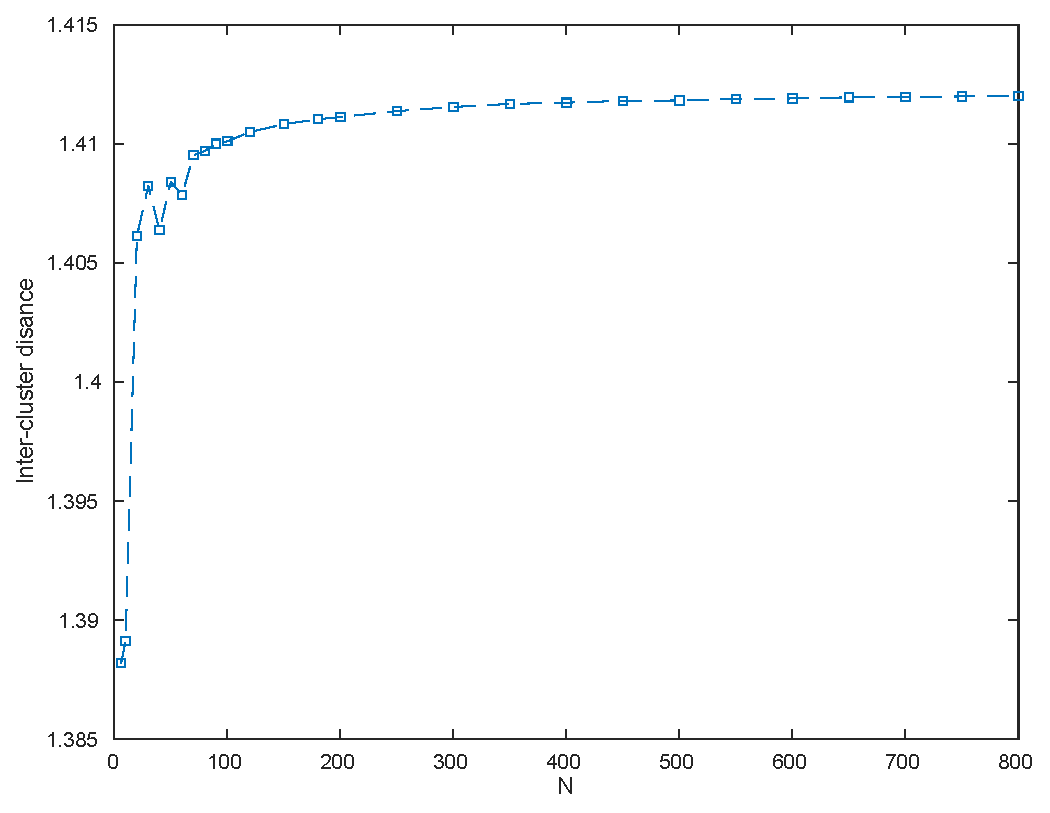
\includegraphics[width = \linewidth]{dvn.eps}
            \caption{Inter-cluster distance for static two cluster state. Simulations were run for various values of \(N\) with \(K = -0.5,J = 0.3,\gamma_1 = 2/3,\gamma_1 = -1/3\). Swarmalators were initially positioned in two equally sized clusters with average phase \(0\) and \(\pi\) and simualtions were run for \(T = 300\) time steps.}
            \label{fig:dvn}
        \end{figure}
        \begin{figure}[h!]
            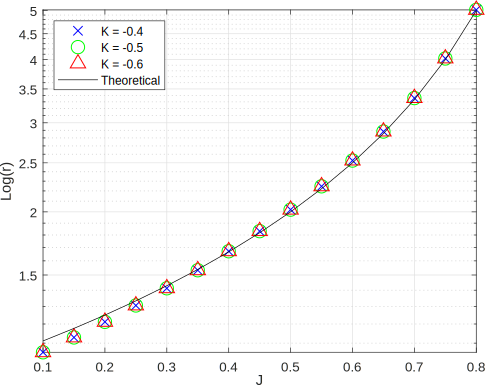
\includegraphics[width = \linewidth]{interClust.eps}
            \caption{Inter-cluster distance for varying K. Simulations were run for various values of \(K\) and \(J\) for \(N = 800\). The black line shows the theoretical prediction as per Eq.\ref{eq:eqdist}. The figure justifies that inter-cluster distance is independent of \(K\).}
            \label{fig:KvJ}
        \end{figure}
        Also, from Eq.\ref*{eq:eqdist}, we realize that for \(J \geq 1\) the two clusters move to infinity. 
    }
    \subsection{Stability of Static two cluster state}
    {

    }
}

\section{Periodic motion of Rogues}

\section{Circular ring state}
{
    In a search for more stable states, we encountered a possibly stable state which could be achieved with careful arrangement of swarmalators. It can be achieved by placing a swarmalators around a circle with a single swarmalator in the center. The circumferential swarmalators have phase \(\pi\) off from the center. 
}

\section{Phase Variation within the clusters}

\noindent

\section{Simplified model}

\section{Front end application}

\section{Conclusion}


\section{References}
% CHALMERS UNIVERSITY OF TECHNOLOGY (2019). Methodology for Topology and Shape Optimization: Application to a Rear Lower Control Arm. [online] Sweden. Available at: \url{https://www.chalmers.se/SiteCollectionDocuments/Produkt-%20och%20produktionsutveckling/Nationell%20kompetensarena%20kring%20produktoptimering/Methodology_for_Topology_and_Shape_Optimization_report.pdf [Accessed 5 Nov. 2019].}

\end{document}